\documentclass[./4_GeneralApproach.tex]{subfiles}
\graphicspath{{\subfix{../../Images}}}

\begin{document}
Fig. \ref{fig:contract_based_architecture} summarises the contract-based specification of the general system.

\begin{figure}[htp]
    \centering
    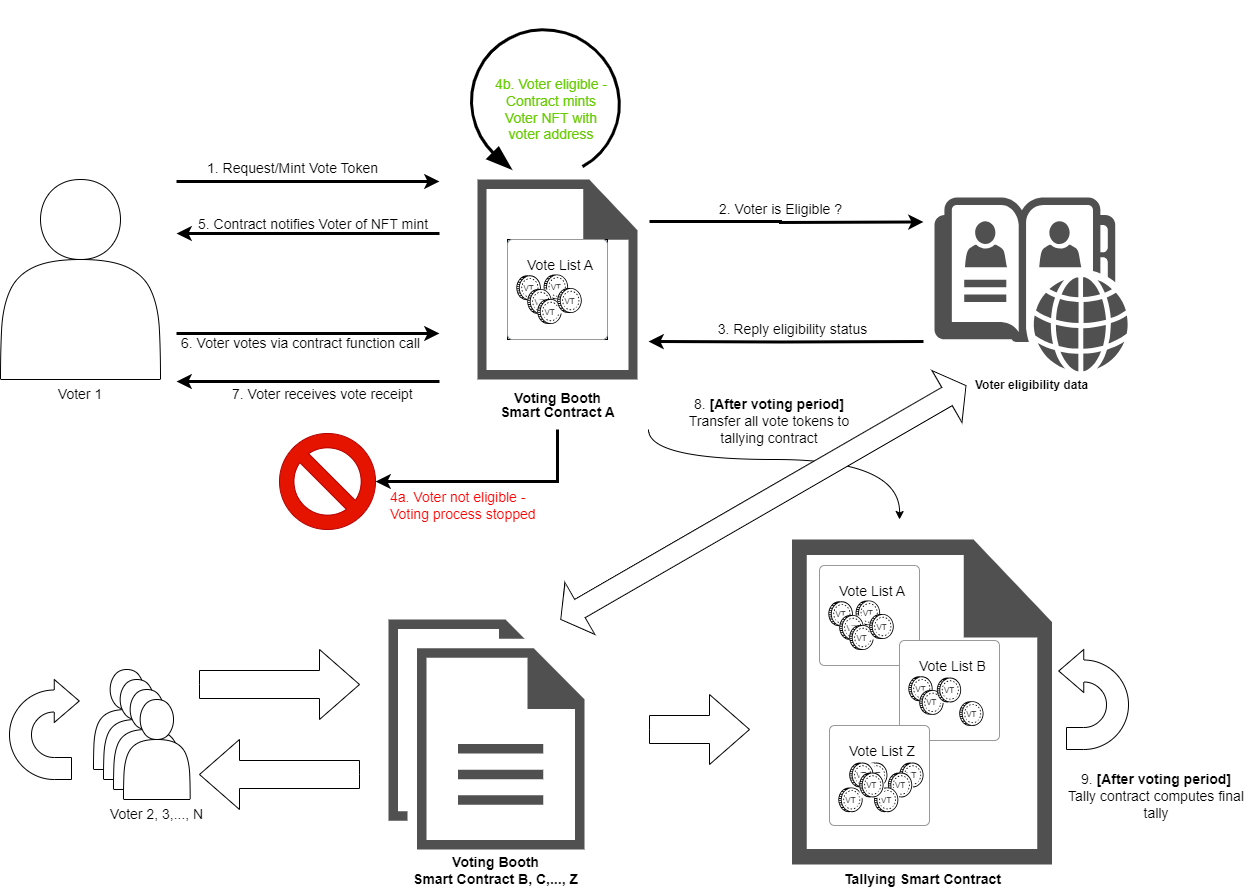
\includegraphics[width=0.7\textwidth]{../Images/02_contract_based_solution.png}
    \caption{Contract-based version of the e-voting system proposed.}
    \label{fig:contract_based_architecture}
\end{figure}

The crucial aspect to take into account with this version is how contract-based blockchains store smart contract-related data. All data related to a smart contract, from token ownership records to token metadata (in the case of NFT-generating smart contracts), is stored "into" the contract, i.e., in a block array referenced from the block where the contract was deployed.



The details of how this storage is processed are beyond the scope of this document, but this fact exposes a security issue that requires addressing since contract-based blockchains are quite common, and we intend to implement this version of the solution in Ethereum, perhaps the best example of such a blockchain.
\par
Encrypting the data using the public key from an asymmetrical encryption key pair is the most obvious solution and one we intend to explore to mitigate this issue. Regardless of the simplicity of the approach, there are several options on how to employ this encryption layer that require careful consideration first.
\end{document}